\documentclass[12pt,preprint]{aastex}

% has to be before amssymb it seems
%\usepackage{color,hyperref}
%\definecolor{linkcolor}{rgb}{0,0,0.5}
%\hypersetup{colorlinks=true,linkcolor=linkcolor,citecolor=linkcolor,
%            filecolor=linkcolor,urlcolor=linkcolor}
%\usepackage{amssymb,amsmath}

\usepackage{color}
\usepackage{url}
\usepackage{graphicx}
\graphicspath{{figures/}}

% For Python code
\usepackage{listings}
\definecolor{lbcolor}{rgb}{0.9,0.9,0.9}
\lstset{language=Python,
        basicstyle=\footnotesize\ttfamily,
        showspaces=false,
        showstringspaces=false,
        tabsize=2,
        breaklines=false,
        breakatwhitespace=true,
        identifierstyle=\ttfamily,
        keywordstyle=\bfseries\color[rgb]{0.133,0.545,0.133},
        commentstyle=\color[rgb]{0.133,0.545,0.133},
        stringstyle=\color[rgb]{0.627,0.126,0.941},
    }

% Draft watermark:
\usepackage{draftwatermark}
\SetWatermarkLightness{0.9}
\SetWatermarkScale{4}

% Some macros
\newcommand{\todo}[1]{{\color{red} [TODO: #1]}}
\newcommand{\foreign}[1]{{\it #1}}

\newcommand{\apriori}{\foreign{a priori}}
\newcommand{\adhoc}{\foreign{ad hoc}}
\newcommand{\etal}{\foreign{et\,al.}}
\newcommand{\etc}{\foreign{etc.}}

\newcommand{\Fig}[1]{Figure~\ref{fig:#1}}
\newcommand{\fig}[1]{\Fig{#1}}
\newcommand{\figlabel}[1]{\label{fig:#1}}
\newcommand{\Eq}[1]{Equation~(\ref{eq:#1})}
\newcommand{\eq}[1]{\Eq{#1}}
\newcommand{\eqlabel}[1]{\label{eq:#1}}
\newcommand{\Sect}[1]{Section~\ref{sect:#1}}
\newcommand{\sect}[1]{\Sect{#1}}
\newcommand{\App}[1]{Appendix~\ref{sect:#1}}
\newcommand{\app}[1]{\App{#1}}
\newcommand{\sectlabel}[1]{\label{sect:#1}}


\begin{document}

\title{A Few Great Grads Discover Mysterious Stars}

\newcommand{\uwastro}{1}
\author{Graduate X. Student \altaffilmark{\uwastro}}
\author{{\v Z}eljko Ivezi{\'c}\altaffilmark{\uwastro}}
\altaffiltext{\uwastro}{Department of Astronomy, University of Washington}


\begin{abstract}
This paper describes some pretty fancy analysis of APOGEE data. 
The Python implementation of our analysis, along with code to fully reproduce the results
reported here, is available on GitHub.
\end{abstract}

\keywords{
    methods: data analysis ---
    methods: statistical
}

\section{Introduction}
\sectlabel{introduction}

Many types of students are good, but graduate students are the best.

A weakness of this teacher is his poor sense of humor.

\subsection{Grand Plan}

\begin{itemize}
\item  Collaborative work: two teams working on two problems based on APOGEE-ASPCAP 
data\footnote{See http://www.sdss.org/dr12/irspec/}. 
\item Using abundances for 15 elements (allStar file), we will study the variation of their 15-D distribution in 
the 3D XYZ space, as a function of stellar population (halo, thin disk, thick disk); we will use 
Extreme Deconvolution method to quantify the 15-D distributions, see astroML Book Figures 6.11 and 6.12 
\item Using spectra (apStar files), we will run PCA, ICA and NMF methods on them, see astroML Book 
Figures 7.4, 7.6 and 7.7
\end{itemize}    

\begin{itemize}
\item The first step: define the teams, and within each team assign responsibilities for 
\begin{enumerate}
\item learning about the data properties and starting a ``paper'' with a brief Introduction about APOGEE and data properties;  
\item learning about how to download and access data (including writing python code);  
\item learning about how to (modify and) run appropriate astroML tools; 
\item writing analysis summary (including plots) for the ``paper'' 
\end{enumerate}
\end{itemize}    


In \sect{brief_overview} we provide a brief overview of APOGEE.


\section{Brief Overview of APOGEE}
\sectlabel{brief_overview}

\subsection{Initial Analysis}
\sectlabel{initialAnalysis}

I made a pretty plot using APOGEE file {\it allStar-v603.fits}, see \fig{basic_example}. 
You can make it too by running (.py file is in /Project3 directory in github repo):

\begin{lstlisting}
>ipython allStarAnalysis.py
\end{lstlisting}

I also needed to convert png file format to pdf...

\begin{figure}
  \centering
  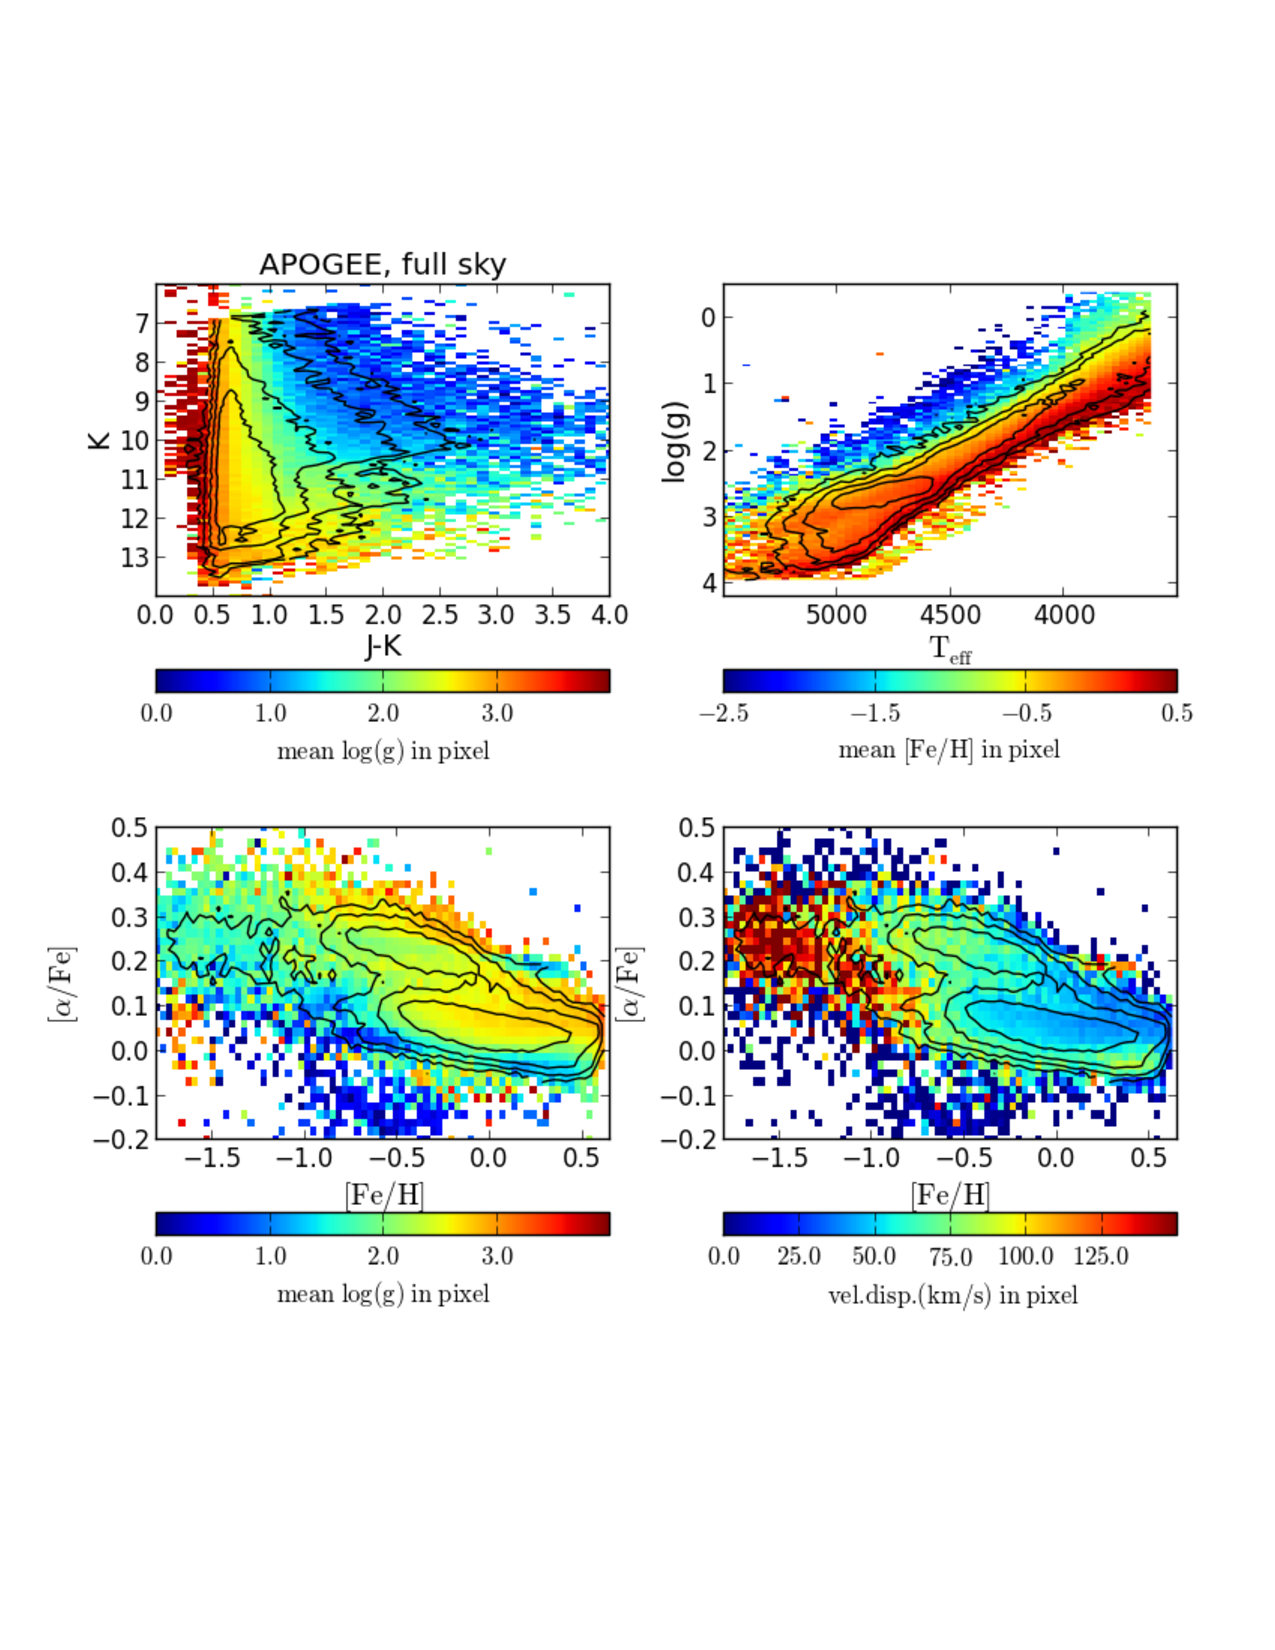
\includegraphics[width=\textwidth]{apogee1.pdf}
  \vskip -1.5in
  \caption{
    An illustration of adding a figure. I made this figure as described in \sect{initialAnalysis}
  }
  \figlabel{basic_example}
\end{figure}


I love reading \citet{Ivezic08LSST}. See why in \sect{discussion}.



\section{Discussion and Conclusion}
\sectlabel{discussion}

Because it's such a nice paper! 

Btw, gory details are in \sect{otherstuff}. 

And yes, given how much these students accomplished, it's not obvious that 
they will not earn their PhDs! 

{\it Acknowledgements:} The authors thank GitHub for providing free academic accounts which were essential 
in the development of this work. We also love SDSS and APOGEE people. 


\bibliographystyle{apj}
\bibliography{paper}


\appendix
\section{Appendix}
\sectlabel{otherstuff}

Here we put gory details that are needed, but break the flow of the paper. 

\end{document}
